\documentclass[oneside,a4paper,11pt]{memoir}
\usepackage[hidelinks]{hyperref}
\usepackage{mathpartir}
\usepackage{listings}
\usepackage{amsmath}
\usepackage{amssymb}
\usepackage{xcolor}
\usepackage{tikz}
\usepackage{subcaption}
\usepackage{mscthesis}
\usepackage{todonotes}
\usepackage{adjustbox}

\setlength{\oddsidemargin}{11pt}
\setlength{\textwidth}{430pt}

\definecolor[named]{oasicsGray}{rgb}{0.31,0.31,0.33}
\definecolor[named]{oasicsBulletGray}{rgb}{0.60,0.60,0.61}
\definecolor[named]{oasicsLineGray}{rgb}{0.51,0.50,0.52}
\definecolor[named]{oasicsLightGray}{rgb}{0.85,0.85,0.86}
\definecolor[named]{oasicsYellow}{rgb}{0.99,0.78,0.07}

\lstset{basicstyle=\small\ttfamily,%
	backgroundcolor=\color{oasicsLightGray},%
	frame=single,framerule=0pt,xleftmargin=\fboxsep,xrightmargin=\fboxsep,
	tabsize=4, 
	escapeinside={`}{`}}


\usepackage{scopegraph}

\makeatletter
\newcommand\@eatpar{\@ifnextchar\par{\expandafter\@eatpar\@gobble}\relax}
\newcommand{\figuresection}[2][]{%
	\par%
	{\sffamily\bfseries #2}\hfill{#1}%
	\smallskip%
	\@eatpar}
\makeatother


\title{Dependently Typed Languages in Statix}
\subtitle{Version of \today}
%\subtitle{Master's Thesis}
\author{Jonathan Brouwer}
\authoremail{\url{j.t.brouwer@student.tudelft.nl}}
\birthplace{Sneek, the Netherlands}
\studentid{4956761}
\coverpicture{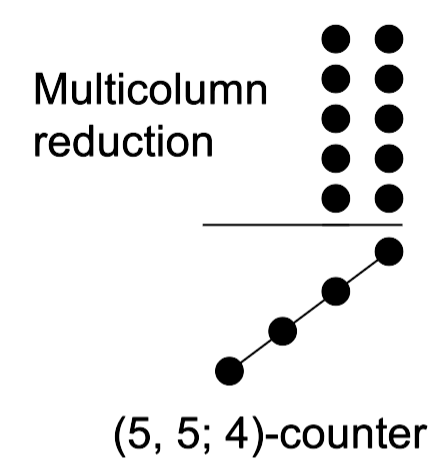
\includegraphics[width=13cm]{./img/cover.png}}
\colophon{\noindent
	\copyright{} \the\year{} \: \theauthor. \\[1em]
	The source code for this thesis can be found online: \\
	\url{https://github.com/JonathanBrouwer/master-thesis}
}

\begin{document}
	
\frontmatter
\thispagestyle{empty}
\maketitle
\null\newpage
\makeformaltitlepages{\noindent Static type systems can greatly enhance the quality of programs, but implementing a type checker for them is challenging and error-prone. The Statix meta-language (part of the Spoofax language workbench) aims to make this task easier by automatically deriving a type checker from a declarative specification of the type system. However, so far Statix has not been used to implement a type system with dependent types, an expressive class of type systems which require evaluation of terms during type checking. 

In this thesis, we present a specification of a simple dependently typed language in Statix, and discuss how to extend it with several common features such as inductive data types, universes, and inference of implicit arguments. While we encountered some challenges in the implementation, our conclusion is that Statix is already usable as a tool for implementing dependent types.}

\cleardoublepage\tableofcontents
	
\mainmatter
% Commands used
\newcommand{\scope}[2]{\langle#1 \: | \: #2\rangle}
\newcommand{\bhr}[3]{ #1 \: #2 \underset{\beta h}{\Rightarrow} #3 }
\newcommand{\toe}[3]{ \scope{#1}{#2} : #3 }
\newcommand{\bred}[3]{ \scope{#1}{#2} \underset{\beta}{\Rightarrow} #3 }
\newcommand{\beq}[2]{ #1 \underset{\beta}{=} #2 }
\newcommand{\co}[1]{ \mathsf{#1} }

\chapter{Introduction}

Type checking programming languages is commonly done by writing a type checker in a general purpose language. This requires a lot of effort, and it is easy to make mistakes. In this thesis we will specifically focus on dependently typed languages, which differ from other languages because they allow types to be parameterized by values. This allows types to express properties of values that cannot be expressed in a simple type system, such as the length of a list or the well-formedness of a binary search tree. This expressiveness also makes dependent type systems more complicated to type check, since deciding equality of types requires normalization of the terms they are parameterized by. 

Instead of writing the type checker in a general purpose language, in this thesis we will systematically derive a type checker from a high-level, declarative specification. This allows for a cleaner implementation that is easy to extend and maintain.

We will do this using the Spoofax language workbench, which is a collection of tools that can derive a parser and type checker from a high level specification of the language~\cite{spoofax}. When working with the Spoofax workbench, the Statix meta-language can be used for the specification of static semantics~\cite{scopes_as_types}. It is a declarative language that uses inference rules to define static semantics. Statix aims to cover a broad range of languages and type systems. However, no attempts have been made yet to express a dependently typed language in Statix until now. 

\section*{Contributions}
This goal of this thesis is to investigate how well Statix is fit for the task of defining a simple dependently-typed language. We want to investigate whether typical features of dependently typed languages can be encoded in Statix. The goal is not only to show that Statix can implement it, but also that the implementation is concise.

The technical contributions of this thesis are the following:
\begin{itemize}
	\item We present a implementation of the Calculus of Constructions, a lambda calculus with dependent types, in Statix (Chapter~\ref{chap:baselang})
	\item We show the language is easily extendable, by extending it with booleans among other features (Chapter~\ref{chap:bools})
	\item We show how to add inference of implicit arguments to the implementation (Chapter~\ref{ch:inference})
	\item We show how to add support for inductive datatypes to the implementation (Chapter~\ref{ch:datatypes})
	\item We show how to add support for universes to the implementation (Chapter~\ref{ch:universes})
\end{itemize}

\section*{Discussions}

Furthermore, the thesis contains some discussions:
\begin{itemize}
	\item We discuss how well semantic code completion works for our language (Chapter \ref{chap:editor-services})
	\item We compare our implementation with an implementation of the same language in Haskell (Chapter \ref{ch:comp-haskell}) and LambdaPi (Chapter \ref{ch:comp-lambdapi})
	\item We discuss how Spoofax can be improved to better support implementing dependently typed languages (Chapter \ref{ch:ergonomics})
	\item We discuss related work (Chapter \ref{ch:relatedwork}) and future work (Chapter \ref{ch:conclusion})
\end{itemize}

Before explaining these contributions, we provide background information on Spoofax and Statix (Chapter \ref{chap:bg-dp}) and the Calculus of Constructions (Chapter \ref{chap:bg-spoofax}).




% !TEX root = document.tex
\chapter{\label{chap:bg-spoofax}Background: Spoofax}

The Spoofax Language Workbench \cite{spoofax} is a platform to develop domain-specific and
general-purpose programming languages. Each aspect of the language is defined in one of three metalanguages, each with their own purpose. From these languages Spoofax generates a parser, type checker and other useful tools. 

The metalanguage SDF3 is used to define the syntax of the language \cite{sdf3}, which is then parsed using Spoofax's SGLR parser \cite{sdf3_parser}. The parser produces a abstract syntax tree in the ATerm format \cite{aterm}. A pretty printer is also generated based on this syntax definition. 

Next, the metalanguage Statix \cite{scopes_as_types} is used to define the static semantics of the language. It uses scope graphs to represent binding and typing information of the language. How this works is discussed in section \ref{sec:statix}.

Finally, Stratego \cite{stratego} is used to define program transformations, using rewrite rules. This can be used for modifications to the AST, but also to build transformations to a different language (such as compiling to assembly). 

\section{\label{sec:statix} Statix and Scope graphs}

In Statix, scope graphs are used to represent a programs name and type information \cite{scopes_as_types}. A scope graph is a graph that consists of the following components:

\begin{itemize}
	\item \textit{Scopes} represent "a region in a program that behaves uniformly with respect to name resolution". These scopes are modeled as nodes in the graph. Its graph representation is shown in \autoref{fig:graph-notation-scope}.
	\item \textit{Labeled, directed edges} model visibility relations between scopes. For example, $\scopet{1} \scopeedget[\lblt{P}] \scopet{2}$ indicates that the graph contains an edge from \scopet{1} to \scopet{2} with label \lblt{P}. Its graph representation can be seen in \autoref{fig:graph-notation-edge}.
	\item \textit{Declarations} model a datum (a piece of information, like the type of a variable) under a relation symbol in a scope. Its textual notation is $\scopet{1} \typeedget[rel] d$, meaning datum $d$ is declared in scope $\scopet{1}$ under relation \textit{rel}. Its pictorial equivalent is shown in \autoref{fig:graph-notation-data}.
\end{itemize}

\begin{figure}[!h]
	\begin{framed}
		\begin{subfigure}{0.2\linewidth}
			\centering
			\begin{tikzpicture}[scopegraph, node distance = 5em and 3.0em]
				\node[scope] (s1) {$1$};
			\end{tikzpicture}
			\caption{Scope}
			\label{fig:graph-notation-scope}
		\end{subfigure}
		\begin{subfigure}{0.4\linewidth}
			\centering
			\begin{tikzpicture}[scopegraph, node distance = 5em and 3.0em]
				\node[scope] (s1) {$1$};
				\node[scope, right of = s1] (s2) {$2$};
				\draw (s1) edge[lbl={P}] (s2);
			\end{tikzpicture}
			\caption{Edge}
			\label{fig:graph-notation-edge}
		\end{subfigure}
		\begin{subfigure}{0.4\linewidth}
			\centering
			\begin{tikzpicture}[scopegraph, node distance = 5em and 3.0em]
				\node[scope] (s1) {$1$};
				\node[type, right of = s1] (s2) {$\texttt{x : INT()}$};
				\draw (s1) edge[type, lbl={rel}] (s2);
			\end{tikzpicture}
			\caption{Data}
			\label{fig:graph-notation-data}
		\end{subfigure}
	\end{framed}
	\caption{Scope Graph notation}
\end{figure}

Information can be retrieved from scope graphs using \textit{queries}. A query from a scope traverses the scope graph to find datums that match certain conditions. The result of a query is a list of (path, datum) tuples. A query has several parameters:
\begin{itemize}
	\item The relation to query. Only datums declared under this relation will be returned by the query.
	\item Path well-formedness condition: a regular expression of labels that specifies which paths are well-formed. Only datums that are reached through a path whose edge labels are in the language described by the regular expression are included in the query result.
	\item A match predicate, taking a single datum as input. Only datums that satisfy this predicate will be included in the query result. Its default value is \verb|true|, meaning that all datums under the specified relation that satisfy the path well-formedness condition are returned.
	\item Result comparison parameters:
	\begin{itemize}
		\item A strict partial order on paths, described by less-than relations on labels. This relation defines a prefix-order on paths.
		\item A `shadow' predicate, which takes two datums as input. Its default value is \verb|false|, meaning that no shadowing is performed.
	\end{itemize}
	When the result set contains multiple datums, and it holds for a datum $d$ that there exists another datum $d'$ which path is strictly smaller that $d$, and the shadow predicate holds, then $d$ is removed from the result set.
\end{itemize}

% CREDIT FOR THIS EXPLANATION TO ARON ZWAAN
% HOW TO CREDIT?
% !TEX root = document.tex
\chapter{\label{chap:bg-dp}Background: Dependent Types}

This chapter will explain the concepts behind dependent types. Readers already familiar with dependent types are recommended to only skim through this chapter.

\section{What are Dependent Types?}

A dependent type system is a type system in which types may depend on values. This means it is possible to have a type such as \verb|Vec n|, which is a vector of exactly length \verb|n|. Note that the value of \verb|n| does not have to be known at compile time, it is therefore more powerful than functions that can be polymorphic over a value.

The biggest advantage of dependent types is that they increase the expressiveness of a type system, for example:
\begin{lstlisting}
append : (A : Type) -> (n : Nat) -> Vec A n -> Vec A n -> Vec A (n + n)
\end{lstlisting}
A \verb|Vec A n| is a list with elements of type \verb|A| that is exactly length \verb|n| (an integer, which is a value!). This append function appends two \verb|Vecs| of equal length, returning a \verb|Vec| of length \verb|n + n|. This is an example of a type-level expression.

In dependent type systems we can use the Curry-Howard Correspondence to prove properties of our code~\cite{chc}. Under this correspondence, types correspond to propositions and a term of a type correspond to a proof of a proposition. Thus if our type system is type-sound\footnote{The type system we will define in chapter~\ref{chap:baselang} is not type-sound, we will fix this by introducing universes in chapter~\ref{ch:universes}.}, that is, we cannot create a term of an empty type, then we can use our type systems to prove things. The type checker will then verify that our proofs are correct.

\section{The Calculus of Constructions}

The lambda cube is a framework to categorize programming languages based on whether terms and types can depend on each other~\cite{lambda_cube}. Specifically, it categorizes languages on three axes: \footnote{Note that the "Terms can depend on terms" axis is missing, this is because a language where terms cannot depend on terms cannot compute anything and is thus pretty useless.}

\begin{enumerate}
	\item Terms can depend on types. This corresponds to type-polymorphic (generic) functions. For example, it allows us to define the polymorphic identity function:
	\begin{lstlisting}
id : (T : Type) -> T -> T
	\end{lstlisting}
	\item Types can depend on types. This corresponds to type-polymorphic (generic) datatypes. For example, it allows to the define the \verb|List T| type, a list with items of type T.
	
	\item Types can depend on terms. This corresponds to dependent types.
\end{enumerate}

The \textit{Calculus of Constructions} is the language that has all three of these features. Now that we have explained the concepts behind Spoofax and dependent types, we will further explain the Calculus of Constructions and implement it in Spoofax in chapter~\ref{chap:baselang}. Then in the chapters after that, we will extend the language with more features.

\chapter{Calculus of Constructions in Statix}
\label{chap:baselang}

In this section, we will describe how to implement a dependently typed language in Statix. In section \ref{sec:coc-syntax} we will describe the syntax of the language, then in section \ref{sec:coc-scopes} we will describe how scope graphs are used to type check the language. Section \ref{sec:coc-dynsyms} describes the dynamic semantics of the language, and finally \ref{sec:coc-typecheck} how to type check the language. This chapter is the main contribution of this thesis.

\section{The Language}
\label{sec:coc-syntax}

The base language that has been implemented is the Calculus of Constructions~\cite{Coquand_Huet_1988}. One extra feature was added that is not present in the Calculus of Constructions: let bindings. Let bindings could be desugared by substituting, but this may grow the program size exponentially, so having them in the language is useful. The concrete syntax (written in SDF3~\cite{sdf3}) of the language is available in figure \ref{fig:syntax}.

\begin{figure}[h]
\lstset{language=SDF3}
\begin{lstlisting}
Expr.Type = "Type"
Expr.Var = ID
Expr.FnType = ID ":" Expr "->" Expr {right}
Expr.FnConstruct = "\\" ID ":" Expr "." Expr
Expr.FnDestruct = Expr Expr {left}
Expr.Let = "let" ID "=" Expr ";" Expr
\end{lstlisting}
\lstset{language=base}
\caption{The concrete syntax for the base language. $\co{FnConstruct}$ is a lambda function, $\co{FnDestruct}$ is application of a lambda function.}
\label{fig:syntax}
\end{figure}

There is only one sort: Expr. The syntax definition does not have a separate sort for types, as types may be arbitrary expressions in a dependently typed language. The following constructors exist:
\begin{itemize}
	\item \verb|Type| is the Type of Types.
	\item \verb|Var| is a variable, it uses the lexical sort \verb|ID|, which is defined as \verb|[a-zA-Z\_][a-zA-Z0-9\_]*|.
	\item \verb|FnType| is the type of a function. It assigns a name to its first argument to allow the return type of the function to depend on the argument type. It is right associative, meaning \verb|A -> B -> C| is interpreted as \verb|A -> (B -> C)|. 
	\item \verb|FnConstruct| creates an anonymous function (lambda function).
	\item \verb|FnDestruct| applies a function to an argument. It is left associative, meaning \verb|a b c| is interpreted as \verb|(a b) c|.
	\item \verb|Let| is a let binding. It introduces a substitutable variable.
\end{itemize}

An example program is the following, which defines a polymorphic identity function (an identity function that is generic over its type) and applies it to a function:

\begin{lstlisting}
let f = \T: Type. \x: T. x;
f (T: Type -> Type) (\y: Type. y)
\end{lstlisting}

The type that the function is generic over needs to be explicitly specified. In most languages, generics are inferred, this inference will also be possible in this language after implementing inference in chapter~\ref{ch:inference}.

\section{Scope Graphs}
\label{sec:coc-scopes}

To type check the base language, we need an environment to store information about the names that are in scope at each point in the program. There are two different types of names that we may want to store, names that do not have a known value (only a type), which are names created by function arguments and dependent function types, and names that do have a known value, which are names created by let bindings.\footnote{In non-dependent languages there is no such distinction, but because we may need \emph{the value} of a binding to compare types, this is needed in dependently typed languages.}

In Statix, all this information can be stored in a \emph{scope graph}~\cite{scope_graphs}, as explained in chapter~\ref{chap:bg-spoofax}. We only use a single type of edge, called \verb|P| (parent) edges. We also only have a single relation, called \verb|name|. The relation associates a \verb|NameEntry| with each name in the scope graph. The \verb|NameEntry| can be either a \verb|NType|, which stores the type of a name, or a \verb|NSubst|, which stores a name that has been substituted with a value. The Statix definition of these concepts is given below:
\begin{lstlisting}
constructors
    NType : Expr -> NameEntry
    NSubst : scope * Expr -> NameEntry
relations
    name : ID -> NameEntry
\end{lstlisting}

Next, we will introduce some Statix predicates that can be used to interact with these scope graphs:

\begin{lstlisting}
sPutType  : scope * ID * Expr -> scope
sPutSubst : scope * ID * (scope * Expr) -> scope
sGetName  : scope * ID -> NameEntry
sEmpty    : -> scope
\end{lstlisting}
The \verb|sPutType| and \verb|sPutSubst| predicates generate a new scope given a parent scope and a type or a substitution respectively. These return a scope that represent an environment that has been extended with the new name. To query the scope graph, we use \verb|sGetName|, which will return the closest \verb|NameEntry| with a matching name. Finally, \verb|sEmpty| returns a fresh empty scope.

We define a \emph{scoped expression}, as a pair of a scope and an expression. The scope acts as the environment of the expression, containing all of the context needed to evaluate the expression.

\section{Beta Reductions}
\label{sec:coc-dynsyms}

A unique requirement for dependently typed languages is beta reduction during type checking, since types may require evaluation to compare. Beta reduction is the process of reduction a term to its beta normal form, which is the state where no further beta reductions are possible~\cite{tapl}. It works by matching a term of the form \verb|(\x. b) e|. and substituting \verb|x| in \verb|b| with \verb|e|. Beta reduction applies this rule anywhere in the term, whereas beta head-reduction only applies this rule at the head (outermost expression) of the term, and produces a term in beta-head normal form.

We implemented beta-head reduction using a Krivine abstract machine~\cite{krivine}. The machine can head evaluate lambda expressions with a call-by-name semantics. This is a strategy under which the leftmost, outermost term is always reduced first~\cite{tapl}. It works by keeping a stack of all arguments that have not been applied yet. This turned out to be the more natural way of expressing this compared to substitution-based evaluation relation, which is an alternative we will discuss in section \ref{sec:coc-subst}.

In conventional dependently typed languages, evaluation is often done using De Bruijn indices.  De Bruijn representation~\cite[Section 6.1]{tapl} uses the distance from a binder to identify a variable. In this representation, alpha equivalence is the same as syntactic equivalence, which can simplify the manipulation of terms. However, we chose to use names rather than De Bruijn indices, because scope graphs work based on names. Using De Bruijn indices would also prevent us from using editor services that rely on \verb|.ref| annotations (which are Spoofax annotations that declare one name as being a use of another name that is a definition).

We need to define multiple predicates that will be used later for type checking. First, the primary predicate is \verb|betaReduceHead|, that takes a scoped expression and a stack of applications, and returns a head-normal expression. The scope acts as the environment from~\cite{krivine}, using \verb|NSubst| to store substitutions. All rules for \verb|betaReduceHead| are given in figure \ref{fig:beta-head-reduce-rules}. We use the syntax $\bhr{\scope{s_1}{e_1}}{\overline{p}}{\scope{s_2}{e_2}}$ to express \textit{betaReduceHead((s1, e1), ps) == (s2, e2)}. The $\overline{p}$ in this definition is the argument stack of the Krivine machine. The argument stack is a stack of scoped expressions, which are the arguments that are not yet paired with a matching function. Figure \ref{fig:beta-head-reduce-rules} contains the rules necessary for beta head reduction of the language. One predicate that is used for this is the \verb|rebuild| predicate, which takes a scoped expression and the stack of arguments (of the Krivine machine state) and converts it to an expression by adding \verb|FnDestruct|s. Its signature is:
\begin{lstlisting}
rebuild : (scope * Expr) * list((scope * Expr)) -> (scope * Expr)
\end{lstlisting}

Additionally, we define \verb|betaReduce| which fully beta reduces a term. It works by first calling \verb|betaReduceHead| and then matching on the head, calling \verb|betaReduce| on the sub-expressions of the head recursively.

\begin{figure}[h]
	\figuresection[\fbox{$\bhr{\scope{s_1}{e_1}}{\overline{p}}{\scope{s_2}{e_2}}$}]{Beta head-reduction rules}

	\begin{mathpar}
		% Type rule
		\inferrule{
		} {
			\bhr
			{ \scope{s}{\co{Type}()} }
			{ [] }
			{ \scope{s}{\co{Type}()}}
		}

		% Let rule
		\inferrule{
			\bhr
			{ \scope{ \co{sPutSubst}(s, x, (s, e))}{b} }
			{ \overline{p} }
			{ \scope{ s' } { b' } }
		}{
			\bhr
			{ \scope{ s }{ \co{Let}(x, e, b) } }
			{ \overline{p} }
			{ \scope { s' } { b' } }
		}

		% Var rule - NSubst
		\inferrule{
			\co{sGetName}(s, x) = \co{NSubst}(s_e, e)
			\\ \bhr
			{\scope{s_e}{e}}
			{\overline{p}}
			{\scope{s_{e'}}{e'}}
		}{
			\bhr
			{\scope{s}{\co{Var}(x)}}
			{\overline{p}}
			{\scope{s_{e'}}{e'}}
		}

		% Var rule - NType
		\inferrule{
			\co{sGetName}(s, x) = \co{NType}(t)
		}{
			\bhr
			{\scope{s}{\co{Var}(x)}}
			{\overline{p}}
			{\co{rebuild}(s, \co{Var}(x), \overline{p})}
		}

		% FnType rule
		\inferrule{
		} {
			\bhr
			{\scope{s}{\co{FnType}(x, a, b)}}
			{[]}
			{\scope{s}{\co{FnType}(x, a, b)}}
		}

		% FnConstruct rule - No args
		\inferrule{
		} {
			\bhr
			{\scope{s}{\co{FnConstruct}(x, a, b)}}
			{[]}
			{\scope{s}{\co{FnConstruct}(x, a, b)}}
		}

		% FnConstruct rule - Args
		\inferrule{
			\bhr
			{\scope{\co{sPutSubst}(s, x, p)}{b}}
			{\overline{p}}
			{\scope{s'}{e'}}
		} {
			\bhr
			{\scope{s}{\co{FnConstruct}(x, \_, b)}}
			{(p::\overline{p})}
			{\scope{s'}{e'}}
		}

		% FnDestruct rule
		\inferrule{
			\bhr
			{\scope{s}{f}}
			{(a::\overline{p})}
			{\scope{s'}{e'}}
		} {
			\bhr
			{\scope{s}{\co{FnDestruct}(f, a)}}
			{\overline{p}}
			{\scope{s'}{e'}}
		}
	\end{mathpar}
	\caption{Rules for beta head reducing the Calculus of Constructions}
	\label{fig:beta-head-reduce-rules}
\end{figure}

\section{Beta Equality}
\label{sec:coc-betaeq}

We need to define \verb|expectBetaEq|, which asserts that two scoped expressions are equal under beta reduction. This rule first beta reduces the heads of both sides, and then compares them. If the head is not the same, the rule fails. Otherwise, it recurses on the sub-expressions. One special case is when comparing two \verb|FnConstruct|s. Here we need to take into account alpha equality: two expressions which only differ in the names that they use should be considered equal. We implement this by substituting in the body of the functions, replacing their argument names with a unique placeholder.

This substitution is called \verb|AlphaEqVars : ID * ID -> Expr|. The combination of the ID on the left and right hand side of the equality guarantees that the substitution is unique. In figure \ref{fig:beta-eq-rules} we show how \verb|AlphaEqVars| is used to determine equality of functions.

\begin{figure}[h]
	\figuresection[\fbox{$\beq{\scope{s_1}{e_1}}{\scope{s_2}{e_2}}$}]{Beta equality rules}
	
	\begin{mathpar}
		\inferrule{
		} {
			\beq
			{ \co{AlphaEqVars}(x_1, x_2) }
			{ \co{AlphaEqVars}(x_1, x_2) }
		}
	
		\inferrule{
			\beq{\scope{s_1}{a_1}}{\scope{s_2}{a_2}}
			\\\\ s_1' = \co{sPutSubst}(s_1, x_1, (\co{sEmpty}(), \co{AlphaEqVars}(x_1, x_2)))
			\\\\ s_2' = \co{sPutSubst}(s_2, x_2, (\co{sEmpty}(), \co{AlphaEqVars}(x_1, x_2)))
			\\\\ \beq{
				\scope{s_1'}{b_1}
				}{ 
				\scope{s_2'}{b_2}
			}
		} {
			\beq
			{ \scope{s_1}{\co{FnType}(x_1, a_1, b_1)} }
			{ \scope{s_2}{\co{FnType}(x_1, a_2, b_2)} }
		}
	
		\inferrule{
			\beq{\scope{s_1}{a_1}}{\scope{s_2}{a_2}}
			\\\\ s_1' = \co{sPutSubst}(s_1, x_1, (\co{sEmpty}(), \co{AlphaEqVars}(x_1, x_2)))
			\\\\ s_2' = \co{sPutSubst}(s_2, x_2, (\co{sEmpty}(), \co{AlphaEqVars}(x_1, x_2)))
			\\\\ \beq{
				\scope{s_1'}{b_1}
			}{ 
				\scope{s_2'}{b_2}
			}
		} {
			\beq
			{ \scope{s_1}{\co{FnConstruct}(x_1, a_1, b_1)} }
			{ \scope{s_2}{\co{FnConstruct}(x_1, a_2, b_2)} }
		}
	\end{mathpar}

	\caption{Rules for beta equality in the Calculus of Constructions}
	\label{fig:beta-eq-rules}
\end{figure}

\section{Type Checking}
\label{sec:coc-typecheck}

We will define a Statix predicate \verb|typeOfExpr| that takes a scope and an expression and type checks the expression in the scope. It returns the type of the expression.

\begin{lstlisting}
typeOfExpr : scope * Expr -> Expr
\end{lstlisting}
We can then start defining type checking rules for the language. We introduce a number of judgements for typing and equality together with their counterparts in Statix.
\begin{enumerate}
	\item $\toe{s}{e}{t}$ is the same as \verb|typeOfExpr(s, e) == t|
	\item $\beq{\scope{s_1}{e_1}}{\scope{s_2}{e_2}}$ is the same as \verb|expectBetaEq((s1, e1), (s2, e2))|
	\item $\bhr{\scope{s_1}{e_1}}{\overline{p}}{\scope{s_2}{e_2}}$ is the same as \verb|betaReduceHead((s1, e1), ps) == (s2, e2)| \\ (The same as in section \ref{sec:coc-dynsyms})
	\item $\bred{s_1}{e_1}{e_2}$ is the same as \verb|betaReduce((s1, e1)) == e2|
	\item $\scope{\co{sEmpty}}{e}$ is the same as $e$ (empty scopes can be left out)
\end{enumerate}

One thing to note is that some rules use \verb|betaReduce|. The goal of this beta reduce is to make the term into a term that does not need an environment (by substituting all let bindings). A full beta reduce is not necessary, but this is merely a performance optimization.

The inference rules in figures \ref{fig:beta-head-reduce-rules}, \ref{fig:beta-eq-rules}, and \ref{fig:type-check-rules} can be directly translated to Statix rules. For example, the rule for \verb|Let| bindings in figure \ref{fig:type-check-rules} is expressed like this in Statix:
\begin{lstlisting}
typeOfExpr(s, Let(n, v, b)) = typeOfExpr(s', b) :-
    typeOfExpr(s, v) == vt, sPutSubst(s, n, (s, v)) == s'.
\end{lstlisting}

\begin{figure}[h]
	\figuresection[\fbox{$\toe{s}{e}{t}$}]{Type checking rules}
	\begin{mathpar}
		\mprset{vskip=0.7ex}
		% Type rule
		\inferrule{
		} {
			\toe{s}{\co{Type}()}{\co{Type}()}
		}

		% Let rule
		\inferrule{
			\toe{s}{e}{t_e}
			\\ \toe{\co{sPutSubst}(s, x, (s, e))}{b}{t_b}
		}{
			\toe{s}{\co{Let}(x, e, b)}{t_b}
		}

		\\

		% Var rule - NType
		\inferrule{
			\co{sGetName}(s, x) = \co{NType}(t)
		}{
			\toe{s}{\co{Var}(x)}{t}
		}

		% Var rule - NSubst
		\inferrule{
			\co{sGetName}(s, x) = \co{NSubst}(s_e, e)
			\\ \toe{s_e}{e}{t}
		}{
		 	\toe{s}{\co{Var}(x)}{t}
		}

		% FnType rule

		\inferrule{
			\toe{s}{a}{t_a}
			\\ \beq{t_a}{\co{Type}()}
			\\ \bred{s}{a}{a'}
			\\\\ \toe{\co{sPutType}(s, x, a')}{b}{t_b}
			\\ \beq{t_b}{\co{Type}()}
		} {
			\toe{s}{\co{FnType}(x, a, b)}{\co{Type}()}
		}


		% Force these to be on the same line, using negative spaces
		\!\!\!\!\!\!\!\!\!\!\!\!\!\!\!\!\!\!\!\!\!\!\!\!\!\!\!


		% FnConstruct rule
		\inferrule{
			\toe{s}{a}{t_a}
			\\ \beq{t_a}{\co{Type}()}
			\\ \bred{s}{a}{a'}
			\\\\ \toe{\co{sPutType}(s, x, a')}{b}{t_b}
		} {
			\toe{s}{\co{FnConstruct}(x, a, b)}{\co{FnType}(x, a', t_b)}
		}

		% FnDestruct rule
		\inferrule{
			\toe{s}{f}{t_f}
			\\ \bhr
				{\scope{s}{t_f}}
				{[]}
				{\scope{s_f}{\co{FnType}(x, t_{da}, t_b)}}
			\\\\ \toe{s}{a}{t_a}
			\\ \beq{t_a}{\scope{s_f}{t_{da}}}
			\\ \bred{\co{sPutSubst}(s_f, x, (s, a))}{t_b}{t_b'}
		} {
			\toe{s}{\co{FnDestruct}(f, a)}{t_b'}
	 	}

		\mprset{vskip=0ex}
	\end{mathpar}
	\caption{Rules for type checking the Calculus of Constructions}
	\label{fig:type-check-rules}
\end{figure}

\section{Discussion of a Substitution-Based Approach}
\label{sec:coc-subst}

An alternative for a Krivine machine, which keeps a stack of arguments it has encountered, is a substitution-based relation. This beta-reduces a \verb|FnDestruct| by doing a nested beta-reduction of the function, and substituting into that, as is shown in figure \ref{fig:subst-approach}.

Although these rules look cleaner, they are more complicated to implement, requiring a separate relation to check if \verb|f| is a \verb|FnConstruct| or something else. For the pure calculus of constructions this still works quite well, but when adding inductive datatypes (chapter~\ref{ch:datatypes}) the rules required become a lot more complex than those for a Krivine machine.

An additional benefit of Krivine machines is that the run-time performance of them tends to be a bit better, though this is only a constant factor and not a time-complexity improvement.

\begin{figure}[h]
	\figuresection[\fbox{$\bhr{\scope{s_1}{e_1}}{}{\scope{s_2}{e_2}}$}]{A substitution-based approach for beta reduction}
	\begin{mathpar}
		\mprset{vskip=0.7ex}
		
		\inferrule{
			\bhr
			{\scope{s}{f}}{}
			{\scope{s_{f'}}{\co{FnConstruct}(x, \_, b)}}
			\\ \bhr
			{\scope{\co{sPutSubst}(s_{f'}, x, (s, a))}{b}}{}
			{\scope{s_{b'}}{b'}}
		} {
			\bhr
			{\scope{s}{\co{FnDestruct}(f, a)}}{}
			{\scope{s_{b'}}{b'}}
		}
	
		\inferrule{
			\bhr
			{\scope{s}{f}}{}
			{\scope{s_{f'}}{f'}}
			\\ \nexists x \, e_1 \, e_2. \, \, f' = \co{FnConstruct}(x, e_1, e_2)
		} {
			\bhr
			{\scope{s}{\co{FnDestruct}(f, a)}}{}
			{\scope{s}{\co{FnDestruct}(f, a)}}{}
		}
	
		\inferrule{
		} {
			\bhr
			{\scope{s}{\co{FnConstruct}(x, a, b)}}{}
			{\scope{s}{\co{FnConstruct}(x, a, b)}}{}
		}
		
		\mprset{vskip=0ex}
	\end{mathpar}
	\caption{A substitution-based approach for beta reduction}
	\label{fig:subst-approach}
\end{figure}

We now have an implementation of the Calculus of Constructions in Spoofax. This implementation still has the issue of variable capture, which we will discuss and solve on chapter \ref{chap:namecolls}. Next, from chapter \ref{chap:bools} onward we will show how to extend the language.

% !TEX root = document.tex

\chapter{\label{chap:namecolls}Avoiding Variable Capturing}

We have now implemented the Calculus of Constructions in Statix. The implementation has one big problem, that is variable capture. Variable capture is the phenomenon of free variables in a term becoming bound when a naive substitution happens~\cite{tapl}. This chapter will explore several ways of solving this. 

An example term where this problem occurs is the following: What is the type of this expression (a polymorphic identity function)?
\begin{lstlisting}
\T : Type. \T : T. T
\end{lstlisting}
The implementation so far would tell you it is \verb|T : Type -> T : T -> T| \todo{why is this wrong}. Given the scoping rules of the language, that is equivalent to \verb|T : Type -> x : T -> x|. However, the correct answer would be \verb|T : Type -> x : T -> T|. There is no way of expressing this type without renaming a variable.

\section{In depth: Why does this happen?}

In this section, we will step through the steps that happen during the type checking of the term above, to explain why the incorrect type signature is returned. To find the type, the following is evaluated:

\begin{lstlisting}
typeOfExpr(_, FnConstruct("T", Type(), 
    FnConstruct("T", Var("T"), Var("T")))
)
\end{lstlisting}

\noindent
This first handles the outer \verb|FnConstruct|, it creates a new node in the scope graph, and then type checks the body with this scope.

\begin{lstlisting}
typeOfExpr(s1, FnConstruct("T", Var("T"), Var("T")))
\end{lstlisting}
\begin{tikzpicture}[scopegraph, node distance = 2.5em and 3.0em]
\node[scope] (s1) {$s1$};
\node[type, above of = s1] (s1l) {$\texttt{T : Type()}$};
\draw (s1) edge[type] (s1l);
\end{tikzpicture}

\noindent
The same thing happens, the body of the \verb|FnConstruct| is typechecked with a new scope. Note that \verb|Var("T")| in the type of the second \verb|T| is ambiguous, does it refer to the first or second node?

\begin{lstlisting}
typeOfExpr(s2, Var("T"))
\end{lstlisting}
\begin{tikzpicture}[scopegraph, node distance = 2.5em and 2.5em]
	\node[scope] (s1) {$s1$};
	\node[type, above of = s1] (s1l) {$\texttt{T : Type()}$};
	\draw (s1) edge[type] (s1l);
	
	\node[scope, right of = s1, xshift=5em] (s2) {$s2$};
	\node[type, above of = s2] (s2l) {$\texttt{T : Var("T")}$};
	\draw (s2) edge[type] (s2l);
	
	\draw (s2) edge[] (s1);
\end{tikzpicture}

Finally, we need to find the type of \verb|Var("T")| in \verb|s2|. This finds the lexically closest definition of \verb|T| (the one in s2), which is correct. But the type of \verb|T| is \verb|T|, which does NOT refer to the lexically closest \verb|T|, but instead to the \verb|T| in s1. This situation, in which a type can contain a reference to a variable that is shadowed, is the problem. We need to find a way to make sure that shadowing like this can never happen.

\section{Alternative Solutions}

Now that the problem is clear, we will explore several attempts at a solution that failed, before settling on the final solution in section \ref{scopes_for_names}.

\subsection{De Bruijn Indices}

Almost all compilers that typecheck dependently typed languages use de Bruijn representation for variables~\cite{lean}. Using de Bruijn indices in statix is possible, but sacrifices a lot. Many editor services (renaming, go to definition) require \verb|.ref| annotations (which specify which other name a certain name refers to) to be set on names, and this is not possible if the names are no longer a part of the AST and the scope graph.

\subsection{Uniquifying names}

Another solution that was attempted was having a pre-analysis transformation that gives each variable a unique name. This doesn't work for a variety of reasons. First of all, it doesn't actually solve the problem. Names can be duplicated during beta reduction of terms, so we still don't have the guarantee that each variable has a unique name. Furthermore, this changes the names in the AST, so it breaks editor services in the same was as De Bruijn Indices did.

\subsection{Capture-avoiding substitution}

Anytime that we introduce a new name in a type, we could check if the name already exists in the environment, and if it does, choose a different unique name. This approach is called capture-avoiding substitution by renaming~\cite{capture_avoiding_sub}. This is possible but tedious to implement in Statix. It requires a new relation to traverse through the type and rename. This is also an inefficient solution, as many traversals of the type are needed. This was successfully implemented, but we chose against using it since we found a better solution.

\section{Using Scopes to Distinguish Names}
\label{scopes_for_names}

The solution we found to work best in the end is to change the definition of \verb|ID|. To be precise, at the grammar level we have two sorts, \verb|RID| is a "Raw ID", being just a string. \verb|ID| will have two constructors, one being \verb|Syn|, a syntactical \verb|ID|, referring to the lexically closest match. The second one is \verb|ScopedName|, which is defined below.

\begin{lstlisting}
context-free sorts ID
lexical sorts RID
context-free syntax
   ID.Syn = RID
signature constructors
  ScopedName : scope * RID -> ID
\end{lstlisting}

The \verb|ScopedName| constructor takes a scope and a raw ID. The scope is used to uniquely identify the name. The main idea is that whenever we encounter a syntactical name during type checking, we replace it with a scoped name, so it unambiguous. The scope graph will never have a syntactical name in it. However, when querying the scope graph for a syntactical name, we return the lexically closest name.

\subsection{The example revisited}

In this section, we will step through the steps that happen during the type checking of the term above, with name collisions solved. To find the type, the following is evaluated, note that the names are now wrapped in a \verb|Syn| constructor:

\begin{lstlisting}
typeOfExpr(_, FnConstruct(Syn("T"), Type(),
	FnConstruct(Syn("T"), Var(Syn("T")), Var(Syn("T")))))
\end{lstlisting}

\noindent
The name in the \verb|FnConstruct| is replaced with a scoped name. The scope of the name is the scope that the name is first defined in. We then type check the body with this scope.

\begin{lstlisting}
typeOfExpr(s1, FnConstruct(Syn("T"), Var(Syn("T")), Var(Syn("T"))))
\end{lstlisting}
\begin{tikzpicture}[scopegraph, node distance = 2.5em and 3.0em]
	\node[scope] (s1) {$s1$};
	\node[type, above of = s1] (s1l) {$\texttt{ScopedName(s1, T) : Type()}$};
	\draw (s1) edge[type] (s1l);
\end{tikzpicture}


\noindent
The same thing happens, the body of the \verb|FnConstruct| is typechecked with a new scope. Note that the type of the new \verb|T| now specifies which \verb|T| it means, so it is no longer ambiguous.

\begin{lstlisting}
typeOfExpr(s2, Var(Syn("T")))
\end{lstlisting}
\begin{tikzpicture}[scopegraph, node distance = 2.5em and 2.5em]
	\node[scope] (s1) {$s1$};
	\node[type, above of = s1] (s1l) {$\texttt{ScopedName(s1, T) : Type()}$};
	\draw (s1) edge[type] (s1l);
	
	\node[scope, right of = s1, xshift=18em] (s2) {$s2$};
	\node[type, above of = s2] (s2l) {$\texttt{ScopedName(s2, T) : Var(ScopedName(s1, T))}$};
	\draw (s2) edge[type] (s2l);
	
	\draw (s2) edge[] (s1);
\end{tikzpicture}

Finally, we need to find the type of \verb|T|. This finds the lexically closest definition of \verb|T| (the one in s2), as defined earlier. The type of this \verb|T| is \verb|ScopedName(s1, T)|, which explicitly defined which \verb|T| it is. A name can now never shadow another name, since each scope uniquely identifies a name. The final type of the expression is now:

\begin{lstlisting}
FnType(ScopedName(s1, T), Type(),
	FnType(ScopedName(s2, T), Var(ScopedName(s1, T)), 
		Var(ScopedName(s1, T))))
\end{lstlisting}

\section{Improving the Readability of Types}

Because the expression above, with \verb|ScopedName|s, is not particularly readable, we add a new post-analysis Stratego pass (an AST transformation that runs directly after type-checking) that converts the \verb|ScopedName|s to ticked names. For example, the above would be transformed to:

\begin{lstlisting}
FnType(T, Type(), FnType(T', Var(T)), Var(T)))
\end{lstlisting}
Ticks are added to names where necessary. We do this by following these rules:

\begin{enumerate}
	\item When we encounter a \verb|ScopedName| in a definition, we keep adding ticks to the name until we find a name that has not been used before. 
	\item We define a dynamic rule \verb|Rename :: string -> string| and we store the new name we generated using this rule.
	\item When we encounter a \verb|ScopedName| in a variable, use the \verb|Rename| rule to find what the name was transformed to.
\end{enumerate}

We have now solved the problem of variable capture. In chapter \ref{chap:bools}, we explain how to extend the language further, by extending it with booleans. Then, from chapter \ref{ch:inference} onward we use this method to extend the language with various features.


\chapter{\label{chap:bools}Extending the language}

In this chapter, we will add booleans, postulates and type asserts to the language. The goal of this is to show that this language is easy to extend, and to add some features that make testing the language easier.

\section{Booleans}

This section describes how to add Booleans to the language. We will add the type of booleans \verb|Bool|, \verb|true|, \verb|false| and \verb|if|. The \verb|if| expression is not dependent, it expects both branches to have the same type. An example of a program with booleans: 

\begin{lstlisting}
let and = \x: Bool. \y: Bool. if x then y else false end
\end{lstlisting}
The constructors for the language are:

\begin{lstlisting}
BoolType : Expr
BoolFalse : Expr
BoolTrue : Expr
BoolIf : Expr * Expr * Expr -> Expr
\end{lstlisting}
Then, the rules for beta reducing the language are in figure \ref{fig:bool-rules-beta}. There is one particularly interesting case, that is how to beta-reduce if statements. Converting this rule to Statix is not entirely trivial, since you need to choose which rule to apply based on what \verb|c| evaluates to. A new rule is needed, which has 3 cases. One for if \verb|c| evaluates to true, one for if \verb|c| evaluates to false, and finally a third case for other cases (such as when \verb|c| is a variable that does not have a substitution). These rules are stated below: (Remember that \verb|rebuild| is the rule introduced in chapter \ref{chap:baselang}, which takes a scoped expression and a list of arguments and converts it to an expression by adding \verb|FnDestruct|s)

\begin{lstlisting}
betaReduceHead((s, BoolIf(c, b1, b2)), t) = 
  betaReduceHeadIf(s, betaReduceHead((s, c), []), c, b1, b2, t).
betaReduceHeadIf(s, (_, BoolTrue()), _, b1, _, t) = 
  betaReduceHead((s, b1), t).
betaReduceHeadIf(s, (_, BoolFalse()), _, _, b2, t) = 
  betaReduceHead((s, b2), t).
betaReduceHeadIf(s, _, c, b1, b2, t) = 
  rebuild((s, BoolIf(c, b1, b2)), t).
\end{lstlisting}

\begin{figure}[ht]
\begin{mathpar}
	\inferrule{
	} {
		\bhr
		{ \scope{s}{\co{BoolTrue}()} }
		{ [] }
		{ \scope{s}{\co{BoolTrue}()}}
	}

	\inferrule{
	} {
		\bhr
		{ \scope{s}{\co{BoolFalse}()} }
		{ [] }
		{ \scope{s}{\co{BoolFalse}()}}
	}

	\inferrule{
	} {
		\bhr
		{ \scope{s}{\co{BoolType}()} }
		{ [] }
		{ \scope{s}{\co{BoolType}()}}
	}

	\inferrule{
		\bhr
		{ \scope{s}{c} }
		{ [] }
		{ \scope{s'}{\co{BoolTrue}()} }
		\\\bhr
		{ \scope{s}{b1} }
		{ t }
		{ \scope{s''}{b1'} }
	} {
		\bhr
		{ \scope{s}{\co{BoolIf}(c, b1, b2)} }
		{ t }
		{ \scope{s}{b1'}}
	}

	\inferrule{
		\bhr
		{ \scope{s}{c} }
		{ [] }
		{ \scope{s'}{\co{BoolFalse}()} }
		\\\bhr
		{ \scope{s}{b2} }
		{ t }
		{ \scope{s''}{b2'} }
	} {
		\bhr
		{ \scope{s}{\co{BoolIf}(c, b1, b2)} }
		{ t }
		{ \scope{s}{b2'}}
	}
\end{mathpar}
\caption{Rules for beta head reducing booleans}
\label{fig:bool-rules-beta}
\end{figure}

Next, the rules for type-checking booleans are in figure \ref{fig:bool-rules-typecheck}, which are relatively simple. The if expression checks that both branches have the same type, as it is a non-dependent if statement.

\begin{figure}[ht]
\begin{mathpar}
	\inferrule{
	} {
		\toe{s}{\co{BoolType}()}{\co{Type}()}
	}

	\inferrule{
	} {
		\toe{s}{\co{BoolTrue}()}{\co{BoolType}()}
	}

	\inferrule{
	} {
		\toe{s}{\co{BoolFalse}()}{\co{BoolType}()}
	}

	\inferrule{
		\toe{s}{c}{ct}
		\\\beq{ct}{\co{BoolType}()}
		\\\\
		\\\toe{s}{b1}{tb1}
		\\\toe{s}{b2}{tb2}
		\\\beq{tb1}{tb2}
	} {
		\toe{s}{\co{BoolIf}(c, b1, b2)}{tb1}
	}
\end{mathpar}
\caption{Rules for type checking booleans}
\label{fig:bool-rules-typecheck}
\end{figure}

\section{Postulate}

Next we will add \verb|Postulate| to the language. A postulate declares that there is a variable with a certain type, without specifying a value. Through the view of the Curry-Howard correspondence, this is equivalent to an axiom. At the current stage, this is useful for testing the language. For example, this is a test with a postulate:
\begin{lstlisting}
postulate T : Type;
if true then Bool else T end
\end{lstlisting}
The following rules are used to implement the feature, which translate cleanly to Statix:

\begin{figure}[ht]
	\begin{mathpar}
		\inferrule{
			\bhr
			{\scope{s}{b}}
			{a}
			{\scope{s'}{b'}}
		}{
			\bhr
			{\scope{s}{\co{Postulate}(n, t, b)}}
			{a}
			{\scope{s'}{b'}}
		}
	
		\inferrule{
			\toe{s}{t}{tt}
			\\\beq{tt}{\co{Type}()}
			\\\\\bred{s}{t}{t'}
			\\\toe{\co{sPutType}(s, n, t')}{b}{bt}
		} {
			\toe{s}{\co{Postulate}(n, t, b)}{bt}
		}
	\end{mathpar}
	\caption{Rules for postulates}
	\label{fig:postulate-rules}
\end{figure}

\section{Type Assert}

Finally, we will add \verb|TypeAssert| to the language. This is another feature that is useful for testing. It takes an expression, and it asserts that the expression has a certain type. For example, we can do the following:
\begin{lstlisting}
postulate T : Type;
true : if true then Bool else T end
\end{lstlisting}

Implementing this feature is also straight-forward, we add the following two rules, which translate cleanly to Statix:

\begin{figure}[ht]
	\begin{mathpar}
		\inferrule{
			\bhr
			{\scope{s}{b}}
			{a}
			{\scope{s'}{b'}}
		}{
			\bhr
			{\scope{s}{\co{TypeAssert}(b, t)}}
			{a}
			{\scope{s'}{b'}}
		}
		
		\inferrule{
			\toe{s}{t}{tt}
			\\\beq{tt}{\co{Type}()}
			\\\\\toe{s}{b}{bt}
			\\\beq
			{bt}
			{\scope{s}{t}}
		} {
			\toe{s}{\co{TypeAssert}(b, t)}{bt}
		}
	\end{mathpar}
	\caption{Rules for type assertions}
	\label{fig:typeassert-rules}
\end{figure}


\section{Extensibility of the approach}

Now that a few features have been implemented, we can discuss how easy the language is to extend. The conclusion so far is that it is doable in a clean way. Specifically, the approach for each of the features above was:

\begin{enumerate}
	\item Define the parsing rules for the new feature
	\item Create a new file, \verb|tp_bools.stx| and import this file in the main \verb|type_check.stx| file.
	\item In the new file, define a case for the \verb|betaReduceHead| rule for the constructors that were added. Also define cases for \verb|expectBetaEq| and \verb|betaReduce| if necessary. It is necessary iff the new constructors are not always eliminated by \verb|betaReduceHead|.
	\item In the new file, define a case for the \verb|typeOfExpr| rule for the constructors that were added.
\end{enumerate}

This allows each feature to be isolated to its own file. If we decide that we don't like a feature after all, we can remove it simply by unimporting the file. This problem is similar to the expression problem\cite{expression_problem}, which Statix solves very well.

In the following chapters, we're going to be extending the language further with these more interesting features using this approach:
\begin{itemize}
	\item Inference (chapter \ref{ch:inference})
	\item Inductive Datatypes (chapter \ref{ch:datatypes})
	\item Universes (chapter \ref{ch:universes})
\end{itemize}




\chapter{Term Inference}
\label{ch:inference}

Inference is an important feature of dependent programming languages, that allows redundant parts of programs to be left out. For example, it allows you to infer the arguments of a function, if they can be inferred by the arguments that follow, like here where the type of the argument can be inferred, since we pass it \verb|true| which is a boolean:
\begin{lstlisting}
let id = (\T : Type. \x: T. x);
id _ true
\end{lstlisting}

We call it \emph{term inference} rather than \emph{type inference}, because we can infer values other than types. For example, it can infer that the \verb|_| in this example must be \verb|true|:
\begin{lstlisting}
postulate f: Bool -> Type;
postulate g: f true -> Type;
\x: f _. g x
\end{lstlisting}

\section{Different algorithms for inference}
\label{strength-inference}

There are a lot of different algorithms for inference\cite{typeinference}, some algorithms can solve more inferences than others. One algorithm for unification is \emph{first-order unification}, where if at any point during type checking we assert that $\beq{e_1}{e_2}$ and either $e_1$ or $e_2$ is a free variable, we set the the value free variable to be equal to the value of the non-free variable. There are some situations in which this approach fails, but in most real-world scenarios it works perfectly. For example, it can infer both programs in the introduction of this chapter, but it fails to infer the following program:

\begin{lstlisting}
let f = _;
\x : Type.
\g: (_: (f x) -> Bool).
g true
\end{lstlisting}

We know that \verb|f| is a function from \verb|Type -> Type|, but it fails to infer the value of \verb|f|. Because of the way that \verb|g| is used, the type checker asserts that $\beq{f x}{Bool}$. Since x is declared as a function argument and it is completely free, this means that for any \verb|x|, \verb|f x = Bool|. But the rule above is not powerful enough to derive this, so it fails.

\section{Inference in Statix}
\label{statix-inference}

We would like to avoid implementing an algorithm at all, instead using Statix' built-in first-order unification to do the type inference for us. Implementing an inference algorithm in Statix is theoretically possible but this would be a lot of ugly code (since Statix is not a general-purpose programming language), and the goal is to use Statix in a way that is clean and declarative, not to do optimal inference.

However, we cannot immediately use Statix' built-in first-order unification (which acts in the meta language, Statix) to implement first-order unification in the object language. Ideally when implementing beta equality we would match on $\beq{e_1}{e_2}$ where $e_1$ is a free variable, but Statix does not allow for querying whether variables are free. 

Instead, we will be implementing a novel, less powerful form of first-order unification. This will work by explicitly denoting which variables \emph{could be} free, and explicitly handling these cases in a way that approximates first-order unification. We will denote this algorithm as \emph{approximated first-order unification (AFOU)}.

\section{Implementing AFOU}
\label{implementing-inference}

First, we introduce a new constructor \verb|Infer : Expr -> Expr|, which denotes the variables which could be free. The constructor is introduced when we encounter a \verb|_| variable, a marker that something needs to be inferred.
\begin{lstlisting}
typeOfExpr(s, Var(Syn("_"))) = (Infer(q), qt) :-
	(_, qt) == typeOfExpr(sEmpty(), q).
\end{lstlisting}

Note that the type of \verb|typeOfExpr| has changed, it now returns two expressions, the first being the same expression that was passed in except with \verb|_| variables replaced with \verb|Infer| constructors, and the second being the type.
\begin{lstlisting}
typeOfExpr : scope * Expr -> Expr * Expr
\end{lstlisting}



\section{Analysis of the power of AFOU}
\label{analysing-inference}


\begin{comment}
	

\section{Using Statix' first-order unification for inference}



When an \verb|Infer| needs to be type-checked, the logic is very similar, except that we don't need to generate a new metavariable:

\begin{lstlisting}
typeOfExpr_(s, Infer(q)) = (Infer(q), t) :-
	typeOfExpr_(s, q) == (_, t).
\end{lstlisting}
When we encounter a \verb|Infer| in \verb|betaReduceHead|, we keep it intact, because we still want to know that it is a \verb|Infer| in the \verb|expectBetaEq| rule. 

The \verb|expectBetaEq| is where it gets interesting. We have a rule for each constructor in the language. For simple cases like \verb|BoolTrue|, we assert that \verb|e2| must be equal.
\begin{lstlisting}
expectBetaEq_((s1, e1@BoolTrue()), (_, Infer(e2))) :- e1 == e2.
\end{lstlisting}
For more complicated constructors such as \verb|FnType|, we generate new metavariables for the subexpressions, and assert they it must be beta-equal to the provided ones:
\begin{lstlisting}
expectBetaEq_(
	(s1, e1@FnType(arg_name1, arg_type1, body1)), 
	(_, Infer(e2))) :- {arg_type2 body2}
  e2 == FnType(arg_name1, Infer(arg_type2), Infer(body2)),
  expectBetaEq_((s1, e1), (sEmpty(), e2)).
\end{lstlisting}

Finally, there is a case for if we encounter two \verb|Infer|s. Ideally, we would look at whether one infer is instantiated, and apply the rules above. However, this is not possible since we cannot do such queries in Statix. Instead, we say that they must be exactly equal and we hope for the best. There are situations where this rule fails (where e1 and e2 are beta-equal but not identical), but this works well enough for practical use.
\begin{lstlisting}
expectBetaEq_((_, Infer(e1)), (_, Infer(e2))) :-
    e1 == e2.
\end{lstlisting}
\end{comment}
\chapter{Inductive Data Types}
\label{ch:datatypes}

\section{Introduction to Inductive Data Types}
\label{ch:datatypes:intro}

Another useful feature is support for inductive data types. An example of a simple inductive datatype is the \verb|Nat| type:
\begin{lstlisting}
data Nat : -> Type where
    zero : Nat,
    suc : Nat -> Nat;
\end{lstlisting}
We will design data types to have the same features as in Agda:
\begin{enumerate}
\item Data types may be recursive, that is the data type may take itself as one of the constructor arguments. This can be seen in the definition of \verb|Nat| above.
\item Parameters, which are datatypes that are polymorphic, and are required to be the same for all constructors, such as
\begin{lstlisting}
data Maybe (T : Type) : -> Type where
    None : Maybe T,
    Some : T -> Maybe T;
\end{lstlisting}
\item Indices, which are datatypes that are polymorphic, that may vary from constructor to constructor
\begin{lstlisting}
data Eq : (e1: Bool) (e2 : Bool) -> Type where
    refl : e : Bool -> Eq e e;
\end{lstlisting}
\item We can also combine parameters and indices, for example to create the generic \verb|Eq| type. Note that parameters and indices may also depend on earlier parameters and indices.
\begin{lstlisting}
data Eq (T : Type) : (e1 : T) (e2 : T) -> Type where
    refl : e : T -> Eq e e;
\end{lstlisting}
\item Data types must be strictly positive. This ensures that we cannot make non-terminating programs\footnote{After we add support for universes in chapter \ref{ch:universes}}. For example, the following data type is forbidden, because it refers to itself in a negative position. We will explain exactly how this check works in section \ref{ch:datatypes:positivity}.
\begin{lstlisting}
data Bad : -> Type where
	bad : (Bad -> Bool) -> Bad;
\end{lstlisting}
\end{enumerate}

A difference between Agda and our implementation is that Agda has case matching as a native construct, whereas we chose to use eliminators \todo{Citation}. An eliminator is a function that can be used to case match on a data type. For example, the eliminator of the \verb|Nat| type above is:
\begin{lstlisting}
elim Nat : P: (v: Nat -> Type) -> P Z 
	-> (x: Nat -> P x -> P (S x)) -> n: Nat -> P n
\end{lstlisting}

The general type of an eliminator for a data type \verb|N| is:
\begin{lstlisting}
parameters 
-> P: (indices -> N params indices -> Type) 
-> constructors
-> indices
-> v: N params indices
-> P indices v
\end{lstlisting}
The meaning of all the arguments is:
\begin{itemize}
	\item \verb|parameters| are the parameters of the data type we want to eliminate, since these are constant among all constructors those can be at the start.
	\item \verb|P| is the type that this eliminator will return. It may depend on the value \verb|v| that is eliminated.
	\item \verb|constructors| is a function that eliminates each of the constructors of the datatype. To eliminate a constructor of the form \verb|C : args -> N params indices| it generates a function \verb|args -> P indices (C pars args)|.
	\item \verb|indices| are the indices of the value that is to be eliminated.
	\item \verb|v| is the value that is to be eliminated.
	\item Finally, \verb|P indices v| is the result of the elimination.
\end{itemize}

\section{Type-checking data type declarations}
\label{ch:datatypes:typechecking}

The definition of \verb|type_check| for an inductive data type \verb|N| is, conceptually:
\begin{enumerate}
	\item Create a new scope \verb|s1| whose parent is the scope the declaration was in \verb|s0|.
	\item Declare \verb|N : Params -> Indices -> Type| in \verb|s1|.
	\item \label{datatype-decl}We use a new scope-graph relation \verb|datatype : ID -> Expr| and declare \\ \verb|N : DataType(name, params, indices, constructors)| in \verb|s1| so that we can access information about the data type later.
	
	\item Create a chain of scopes starting in \verb|s1| that will contain a scope for each parameter. We will type-check each next parameter using the previous parameters scope, so that parameters can depend on previous parameters. Call the end of this chain \verb|s2|.
	
	\item Create a chain of scopes starting in \verb|s2| that will contain a scope for each index. We will type-check each next index using the previous index' scope, so that one index can depend on parameters and previous indices. Call the end of this chain \verb|s3|.
	
	\item Create a new scope \verb|s4| with \verb|s1| as the parent which will be the scope that the rest of the program will be type-checked with. Then type-check each constructor with \verb|s2| as scope (so that the constructors can depend on parameters, but cannot depend on indices), and declare the type of that constructor in \verb|s4|. The parameters are automatically added to the type of the constructor.
\end{enumerate}
For example, for the following inductive datatype:
\begin{lstlisting}
data Eq (T : Type) : (e1 : T) (e2 : T) -> Type where
	refl : e : T -> Eq e e;
...
\end{lstlisting}
Figure \ref{scope-graph-eq} shows the scope graph generated by this data type.
\begin{figure}[!h]
	\begin{framed}
		\centering
		\begin{tikzpicture}[scopegraph, node distance = 6.5em and 5em]
			% S0 and S1 node
			\node[scope] (s0) {$s0$};
			\node[scope, below = 2em of s0] (s1) {$s1$};
			\draw (s1) edge[lbl={P}] (s0);

			% S1 declarations
			\node[type, above right=0.5em and 3em of s1, text width=11cm] (ntype) {\texttt{Eq : (T : Type) -> (e1 : T) -> (e2 : T) -> Type)}};
			\draw (ntype) edge[type, lbl={name}] (s1);
			\node[type, below right=0em and 3em of s1, text width=11cm] (ndatatype) {\texttt{Eq : DataType("Eq", [("T", Type())], [("e1", Var("T")), ("e2", Var("T"))], [("refl", ...)])}};
			\draw (ndatatype) edge[type, lbl={datatype}] (s1);
			
			% Path to S3
			\node[scope, below right=4em and 1em of s1] (s2a) {s2};
			\draw (s2a) edge[lbl={P}] (s1);
			\node[type, right=3em of s2a] (ntype) {\texttt{T : Type}};
			\draw (ntype) edge[type, lbl={name}] (s2a);
			
			\node[scope, below=1em of s2a] (s2b) {};
			\draw (s2b) edge[lbl={P}] (s2a);
			\node[type, right=3em of s2b] (ntype) {\texttt{e1 : T}};
			\draw (ntype) edge[type, lbl={name}] (s2b);
			
			\node[scope, below=1em of s2b] (s2c) {s3};
			\draw (s2c) edge[lbl={P}] (s2b);
			\node[type, right=3em of s2c] (ntype) {\texttt{e2 : T}};
			\draw (ntype) edge[type, lbl={name}] (s2c);
			
			% S4
			\node[scope, below = 12em of s1] (s4) {$s4$};
			\draw (s4) edge[lbl={P}] (s1);
			\node[type, right=3em of s4] (ntype) {\texttt{refl : (T : Type) -> (e : T) -> Eq e e}};
			\draw (ntype) edge[type, lbl={name}] (s4);
		\end{tikzpicture}
	\end{framed}
	\caption{The scope graph generated by the Eq data type.}
	\label{scope-graph-eq}
\end{figure}

\section{Type-checking eliminators}

The type of an eliminator was discussed in section \ref{ch:datatypes:intro}. When we type check an \verb|elim N| expression, the following happens:
\begin{enumerate}
	\item Query the scope to find the data type declaration that we created in point \ref{datatype-decl} of section \ref{ch:datatypes:typechecking}. This gives us access to the parameters, indices and constructors of the data type that is being eliminated. 
	\item Using some tedious logic, create the type discussed in section \ref{ch:datatypes:intro}. This ends up being around 100 lines of Statix code.
\end{enumerate}

The second part that needs to be defined is beta reducing an eliminator. During this process, the following happens:
\begin{enumerate}
	\item Query the scope to find the data type declaration that we created in point \ref{datatype-decl} of section \ref{ch:datatypes:typechecking}. This gives us access to the parameters, indices and constructors of the data type that is being eliminated. (Same as during type checking)
	\item Try to split the arguments applied to the eliminator into the groups defined in section \ref{ch:datatypes:intro}. If this fails (because there are not enough arguments), the eliminator cannot be reduced.
	\item Beta head reduce \verb|v|, if this does not result in one of the constructors at the head then the eliminator cannot be reduced. 
	\item 
\end{enumerate}

\section{Positivity Checking}
\label{ch:datatypes:positivity}
	

\chapter{Universes}
\label{ch:universes}

Our language so far has the property that the type of \verb|Type| is \verb|Type|, this is called \emph{type in type}. This allows for \emph{Girard's paradox}, which means that the logic created by this language is inconsistent: we can prove false~\cite{girard}. 

\section{Universes}

The solution to this problem is to introduce universes into the language. We now have the following hierarchy of types:
\begin{lstlisting}
true : Bool : Type 0 : Type 1 : Type 2 : ...
\end{lstlisting}

In the rest of this chapter we will show how universes have been implemented. It turns out to be relatively easy to add this feature to the language, only requiring a few changes.

\section{Implementing Universes in the Calculus of Constructions}

The \verb|Type| constructor has to be changed to \verb|Type : int -> Expr|, taking the universe of the type as an argument. We then need to update all occurrences of \verb|Type| in figure \ref{fig:type-check-rules}. Figure \ref{fig:type-check-rules-universes} contains all the rules that require a change.

The three rules that were changed are:
\begin{enumerate}
	\item The rule for type-checking a \verb|Type| expression. The universe of \verb|Type u| is \verb|u + 1|. 
	\item The rule for type-checking \verb|FnType|. The universe of \verb|FnType| is the maximum of the universe of the argument and return type.
	\item A trivial change to the rule for type-checking \verb|FnConstruct|, which ignores the universe of its argument type.
\end{enumerate}

\begin{figure}[ht]
	\figuresection[\fbox{$\toe{s}{e}{t}$}]{Type checking rules with universes}
	\begin{mathpar}
		\mprset{vskip=0.7ex}
		% Type rule
		\inferrule{
		} {
			\toe{s}{\co{Type}(u)}{\co{Type}(u+1)}
		}
		
		% FnType rule
		\inferrule{
			\toe{s}{a}{t_a}
			\\ \beq{t_a}{\co{Type}(u_a)}
			\\ \bred{s}{a}{a'}
			\\\\ \toe{\co{sPutType}(s, x, a')}{b}{t_b}
			\\ \beq{t_b}{\co{Type}(u_b)}
		} {
			\toe{s}{\co{FnType}(x, a, b)}{\co{Type}(\co{max}(u_a, u_b))}
		}
		
		% FnConstruct rule
		\inferrule{
			\toe{s}{a}{t_a}
			\\ \beq{t_a}{\co{Type}(u_a)}
			\\ \bred{s}{a}{a'}
			\\\\ \toe{\co{sPutType}(s, x, a')}{b}{t_b}
		} {
			\toe{s}{\co{FnConstruct}(x, a, b)}{\co{FnType}(x, a', t_b)}
		}
		
		\mprset{vskip=0ex}
	\end{mathpar}
	\caption{Rules for type checking the Calculus of Constructions with universes}
	\label{fig:type-check-rules-universes}
\end{figure}

\newpage
\section{Implementing Universes with Inductive Data Types}

We change data type declarations such that the universe the datatype lives in is now explicit. For example, the \verb|Nat| type now looks like this, explicitly stating that the type of \verb|Nat| is \verb|Type 0|.
\begin{lstlisting}
data Nat : -> Type 0 where
	zero : Nat,
	suc : Nat -> Nat;
\end{lstlisting}

We need to make the following changes to the type-checking algorithm:
\begin{enumerate}
	\item In point \ref{name-decl} of type-checking data type declarations in section \ref{ch:datatypes:typechecking}, we need to return \verb|Type u| instead of \verb|Type|, where \verb|u| is the declared universe level.
	\item For all constructors, we need to check that the universe of the constructor arguments is smaller than or equal to \verb|u|. This ensures that the datatype does actually live in the universe \verb|u|.
\end{enumerate}

We have now finished the type checker of the language. Next, we will discuss how to implement the back-end of the language.


% !TEX root = document.tex
\chapter{\label{chap:editor-services}Semantic Code Completion}
 
We explored how semantic code completion presented by Pelsmaeker et al.~\cite{codecompletion} applies to dependently typed languages. Code completion is an editor service in IDEs that proposes code fragments for the user to insert at the caret position in their code.

\section{Setup required}
To set up editor services, we followed the steps at \todo{cite} \url{https://spoofax.dev/spoofax-pie/develop/guide/static-semantics/code-completion/}. To be precise, we followed the following steps:
\begin{enumerate}
	\item Add \verb|tego-runtime {}| and \verb|code-completion {}| to the \verb|spoofax.cfg| file, to enable code completion.
	\item Add the following rules to the \verb|main.str2| file, to pre-process and post-process the AST for code completion.
	\begin{lstlisting}
rules
	downgrade-placeholders = downgrade-placeholders-MyLang
	upgrade-placeholders   = upgrade-placeholders-MyLang
	is-inj                 = is-MyLang-inj-cons
	pp-partial             = pp-partial-MyLang-string
	pre-analyze            = explicate-injections-MyLang
	post-analyze           = implicate-injections-MyLang
	\end{lstlisting}
	\item For each rule define a predicate that accepts a placeholder where a syntactic sort is permitted. For our language, those are the following:
	\begin{lstlisting}
expectBetaEq((_, Expr-Plhdr()), _).
expectBetaEq(_, (_, Expr-Plhdr())).
betaReduceHead((_, Expr-Plhdr())) = _.
betaReduce((_, Expr-Plhdr())) = _.
typeOfExpr(_, Expr-Plhdr()) = _.
programOk(Start-Plhdr()).
	\end{lstlisting}
	
\end{enumerate}

\section{How well it works}
In order to get suggestions, we can now insert a placeholder \verb|[[Expr]]| and press \verb|ctrl + space| in the editor to get semantic suggestions.

It works well, only showing completions that are semantically relevant. For example, given the following code it only suggests expressions that can be booleans:
\begin{lstlisting}
let f = \b: Bool. b;
f [[Expr]]
\end{lstlisting}
This would return the following suggestions: (Note that \verb|f| and \verb|Type| are not suggested, since they cannot have type \verb|Bool|)
 \begin{itemize}
 	\item \verb|[[Expr]] [[Expr]]|
 	\item \verb|let [[ID]] = [[Expr]]; [[Expr]]|
 	\item \verb|true|
 	\item \verb|false|
 	\item \verb|if [[Expr]] then [[Expr]] else [[Expr]] end|
 \end{itemize}
\chapter{A comparison with conventional implementations}
\label{ch:comp-haskell}

In this chapter, we implement the language defined in chapter \ref{chap:baselang} in Haskell, and then compare the implementation with the implementation in Statix. We want the design of the implementation in Haskell to be similar to conventional implementations of dependently typed languages, so we can compare the Statix implementation with them.

\section{Defining the AST}
To implement the calculus of constructions in Haskell, we first define the \verb|Expr| datatype. We chose to define the language using De Bruijn indices, since this is the convention when implementing dependently typed languages, and the goal of this implementation in Haskell is to compare the Statix implementation with conventional ones. 
\begin{lstlisting}
data Expr =
	Type
	| Let Expr Expr
	| Var Int
	| FnType Expr Expr
	| FnConstruct Expr Expr
	| FnDestruct Expr Expr
\end{lstlisting}

\section{Defining environments}

Next, we need to decide how we want to store the environment. We still need to store both function arguments and substitutions, which we called \verb|NType| and \verb|NSubst| in chapter \ref{chap:baselang}. We will use the same names, and store the environment as a list, with the head of the list representing De Bruijn index 0. Finally, we define the type of a scoped expression \verb|SExpr|, as a tuple of an environment and an expression.
\begin{lstlisting}
data EnvEntry = NType Expr | NSubst SExpr
type Env = [EnvEntry]
type SExpr = (Env, Expr)
\end{lstlisting}

The way these environments are defined is isomorphic to the way we defined the way we use scope graphs in section \ref{sec:coc-scopes}. Nodes in the scope graph have at most one parent, and each node stores one entry, which is exactly the structure of a list. For example, the following scope graph and list have the same meaning:

\begin{lstlisting}
NType(Var(0)) :: NType(Type()) :: Nil
\end{lstlisting}
\begin{tikzpicture}[scopegraph, node distance = 2.5em and 2.5em]
	\node[scope] (s1) {$s1$};
	\node[type, above of = s1] (s1l) {$\texttt{T : Type()}$};
	\draw (s1) edge[type] (s1l);
	
	\node[scope, right of = s1, xshift=5em] (s2) {$s2$};
	\node[type, above of = s2] (s2l) {$\texttt{x : Var("T")}$};
	\draw (s2) edge[type] (s2l);
	
	\draw (s2) edge[] (s1);
\end{tikzpicture}

The nodes in scope graphs may have multiple children, but we never query the children of a node. We only follow the edges, we don't go in the opposite direction. Similarly, part of a list may be shared, but this is fine in Haskell, since values are immutable. 

Finally, we define the two functions \verb|sPutSubst| and \verb|sPutType| to mimic the Statix relations with the same name.
\begin{lstlisting}
sPutSubst :: Env -> SExpr -> Env
sPutSubst env v = NSubst v : env
sPutType :: Env -> Expr -> Env
sPutType env v = NType v : env
\end{lstlisting}

\section{Defining beta reduction}

Now we want to define beta head reduction. Remember that in Statix, beta head reduction is a relation with the signature
\begin{lstlisting}
betaReduceHead : 
	(scope * Expr) * list((scope * Expr)) -> (scope * Expr)
\end{lstlisting}

In Haskell, a slightly different structure was used. We defined two functions, one returning a \verb|Maybe SExpr| and the other checking if the result \verb|Nothing|, in which case it returns the original expression (unreduced). This structure could also be implemented in Statix, but Haskell makes it a bit easier for us by providing the \verb|Maybe| type and functions on it.
\begin{lstlisting}
brh :: SExpr -> SExpr
brh e = fromMaybe e (brh_ e [])
brh_ :: SExpr -> [SExpr] -> Maybe SExpr
\end{lstlisting}

\section{Comparison}

The base implementations of the language are quite similar. One difference is the way the definitions are clustered\todo{not right word?}. In Statix, one could put each language construct in a separate file, keeping the definitions for that construct together. In the Haskell implementation this is not easily possible\footnote{We could still define a function that then calls the actual implementation in the separate files, but this is still inferior to the Statix implementation.}, since function definitions can not be split over a file. 

Another advantage that Statix has is that it has first-order inference built-in, which makes implementing a basic form of inference as described in chapter \ref{ch:inference} way easier. However, if we want a more complex form of inference then an implementation in Haskell would be better, since it is a more expressive language and it has more libraries available. 

Finally, creating the language in Spoofax automatically gives us editor services such as code highlighting and semantic autocompletion, as dicusssed in chapter \ref{chap:editor-services}. Implementing these in Haskell would require some work.

\chapter{A comparison with implementations in logical frameworks}
\label{ch:comp-lambdapi}

In chapter \ref{ch:inference} we discussed how to implement inference algorithms, and we concluded in section \ref{analysing-inference} that adding equational unification to Statix would make inference algorithms easier to implement. In this chapter we explore this further, by implementing our dependently typed language in a logical framework. 

A logical framework is a language that provides a means to define a type system. There exist several \emph{logical frameworks}, designed specifically for implementing and experimenting with dependent type theories, such as ALF~\cite{MagnussonN93}, Twelf~\cite{PfenningS99}, Dedukti~\cite{BoespflugCH12}, Elf~\cite{pfenning_1991} and Andromeda~\cite{BauerHP20}. Since these tools are designed specifically for the task, implementing the type system takes less effort in them compared to Spoofax, but for other tasks such as defining a parser or editor services they are not as well equipped. 

In this chapter we will be implementing the language defined in chapter~\ref{chap:baselang} in lambdapi, a proof assistant based on the $\lambda \Pi$-calculus modulo rewriting~\cite{BoespflugCH12}. 

\section{Defining Symbols}

We will define a symbol in the meta language (lambdapi) for each construct in the object language. The result is visible in figure \ref{fig:lp-symbols}. We will leave \verb|Let| out of the language for now, it will be discussed separately in section \ref{ch:comp-lambdapi:let}.

\begin{figure}[ht]
\begin{lstlisting}
constant symbol TmSort : TYPE;
symbol TmType : `Π` (a : TmSort), TYPE;

constant symbol Type : TmSort;

constant symbol FnType :
  `Π` (A : TmSort), 
  `Π` (B : TmType A → TmSort), 
TmSort;

symbol FnConstruct :
  `Π` (A : TmSort), 
  `Π` (B : TmType A → TmSort), 
  `Π` (f : `Π` (x : TmType A), TmType (B x)), 
  TmType (FnType A B);

symbol FnDestruct :
  `Π` (A : TmSort), 
  `Π` (B : TmType A → TmSort), 
  `Π` (f : TmType (FnType A B)),
  `Π` (a : TmType A),
  TmType (B a);
\end{lstlisting}
	\caption{Symbols of the Calculus of Constructions}
\label{fig:lp-symbols}
\end{figure}

First, \verb|TmSort : TYPE| is the meta-language type of a type in the object language. So in any place where we say \verb|A : TmSort|, this means \verb|A| is a type in the object language. Next, \verb|TmType : (a : TmSort) -> TYPE| is the meta-language type of a term of type \verb|a| in the object language. So if we have \verb|x : TmType Bool| then \verb|x| is a boolean in the object language. 

Now we will define a symbol for each construct in the language we are defining.
\begin{enumerate}
	\item \verb|Type| is a type.
	\item \verb|FnType| is a type, but it takes two arguments: \verb|A| is the argument type and \verb|B| is the return type, which is allowed to depend on a value of the argument type.
	\item \verb|FnConstruct| takes three arguments: \verb|A| is the argument type, \verb|B| is the return type (allowed to depend on \verb|A| again), and \verb|f| is a function in the meta language of type \verb|x : A -> B x|.
	\item \verb|FnDestruct| takes four arguments: \verb|A| is the argument type, \verb|B| is the return type (allowed to depend on \verb|A| again), a term of type \verb|A -> B| and an argument of type \verb|A|. 
\end{enumerate}

Note that these constructors can only represent type-correct terms, \emph{intrinsically typed} terms. This is useful because it means the meta language does the type checking for us. The disadvantage is that it requires extra information: We need to give \verb|B| for \verb|FnConstruct| and \verb|A| and \verb|B| for \verb|FnDestruct|, which is information we don't have to provide to type-check terms in Statix. These could easily be automatically generated by a type checker but are tedious to specify manually. It seems like it should be possible to infer these, but lambdapi fails to do so. Further research is required to find out why lambdapi does not infer these.

\section{Reduction Rules}

We now define the \emph{reduction rules}, which define how to reduce the language. A rule $a \hookrightarrow b$ states that \verb|a| reduces to \verb|b|. We reduce the constructs in our language to constructors in lambdapi, this is called \emph{embedding} the language. Lambdapi can then evaluate the rules using its own semantics, not requiring any additional rules similar to the ones in figure \ref{fig:beta-head-reduce-rules}. The reduction rules are given in figure \ref{fig:lp-rules}. Each of the constructs is reduced to the corresponding construct in the meta language.

\begin{figure}[ht]
	\begin{lstlisting}
rule TmType Type `$\hookrightarrow$` TmSort;
rule TmType (FnType $A $B) `$\hookrightarrow$` `Π` (x : TmType $A), TmType ($B x);
rule FnConstruct _ _ $f `$\hookrightarrow$` $f;
rule FnDestruct _ _ $f $a `$\hookrightarrow$` $f $a;
	\end{lstlisting}
	\caption{Reduction Rules for the Calculus of Constructions}
	\label{fig:lp-rules}
\end{figure}

\section{\label{ch:comp-lambdapi:let}Defining Let Bindings}

Let bindings require substitution, which is not possible to encode in lambdapi. We can encode a less powerful version of let bindings, which are not substituted but evaluated via functions. The definition of this is given in figure \ref{fig:lp-let}. The body of the let binding is allowed to depend on a value of type \verb|A|, but it is not aware of the exact value \verb|v| of the let binding. 

\begin{figure}[ht]
	\begin{lstlisting}
symbol Let : 
	`Π` (A : TmSort), 
	`Π` (B : TmType A → TmSort), 
	`Π` (v : TmType A),
	`Π` (b : TmType A → TmType (B v)),
	TmType (B v);
rule Let _ _ $v $b `$\hookrightarrow$` $b $v;
	\end{lstlisting}
	\caption{Definition of less powerful Let in lampdapi}
	\label{fig:lp-let}
\end{figure}

One program which would not type-check with this approach is the following. It fails to compile since it cannot know that \verb|b| is a boolean, which is required by the definition of f. \footnote{Assuming we introduce booleans into the language, there are examples that don't require booleans but they are a bit more difficult to understand}.
\begin{lstlisting}
let T = Bool;
\f: Bool -> Bool;
\b: T. f b
\end{lstlisting}


\chapter{Ergonomics of Spoofax}
\label{ch:ergonomics}

Now that we've implemented a feature-rich dependently typed language in Statix, this chapter discusses the experience, and recommends some changes to Statix and Spoofax which might improve the experience. 

\section{Statix}

Statix is a simple language, not supporting too many complex features. This works well in some ways, but having some more features available could improve the experience drastically. Some features that would've helped this project create better code are:

\begin{enumerate}
	\item Allow specifying reduction rules, and then implement equality under reduction in Statix. This feature was discussed extensively in chapter \ref{ch:comp-lambdapi}. This would require extensive changes to the core language of Statix, so this is challenging to implement.
	
	\item Nested constraints: Defining a constraint that can use the metavariables of a parent constraint. This works similar to nested function definitions. For example, for type checking datatypes:
	\begin{lstlisting}
typeOfExpr_(s, DataTypeDecl(n, ps, is, ue, cs, b)) = ... :-

	isStrictlyPositive : (scope * Expr)
	isStrictlyPositive(s, FnType(...)) = ...
	\end{lstlisting}
	The definition of \texttt{isStrictlyPositive} can then use all the metavariables of \\ \texttt{DataTypeDecl} without having to explicitly pass them. This feature could be desugared by moving the relation to the global scope and explicitly passing the metavariables of the parent constraint when it is used.
	
	\item Generic constraints. For example, we created two separate relations for reversing lists of different types, making these one generic function would have been better. This was the only case where this feature would have been useful for this thesis, but it may be more useful for other work. This could be implemented by monomorphization or by changing the core language. 
\end{enumerate}

\section{Spoofax}

Next we will describe our experience with Spoofax as a whole. 

\begin{enumerate}
	\item Spoofax is still slow, even though its performance has improved over the past years. On a high-end computer\footnote{Intel i7 6700k @ 4.2GHz, 16 GB Ram @ 2133MHz, Arch Linux @ Jan 2023, Spoofax 3 v0.19.2}, we took the following measurements.
	\begin{itemize}
		\item Full build (non-incremental) takes 55 seconds
		\item Incremental build changing only one Statix file takes 5 seconds
		\item Running all 171 tests takes 18 seconds
	\end{itemize}
	While these numbers are not unworkably high, they are still magnitudes higher than the implementation in Haskell (chapter~\ref{ch:comp-haskell}) and other general-purpose languages. Improving these numbers would make the experience better.
	
	\item The SPT testing DSL works very well, it makes writing integration tests very easy. However, support for unit tests is still lacking. The way to create unit tests for the type checker is using Statix tests, allowing assertions on specific relations. But these tests are not integrated with SPT tests (they don't even reside in the test folder) and there is no way to run all Statix tests, to ensure no regressions happened. Ideally there would be one button that runs all SPT and Statix tests.
	
	\item Debugging Statix is still quite tedious. When we have a constraint that does not do what we expect it to do (ie. we have a failing Statix test), one either has to stare at its definition until they figure out the problem, or start unfolding the definitions of the constraints into the Statix test, finding out which part of the definition is misbehaving and repeating the unfolding. Having support for a debugger would help tremendously with this.
	
	The way that this debugger could work is that you could start by entering a certain constraint \verb|typeCheck(...)|, the debugger would then show the current value of each metavariable in scope, and each constraint that is yet to be expanded. Since there is no fixed evaluation order in Statix, we could even allow the programmer to choose which constraint is evaluated next, which then generates more constraints.
\end{enumerate}


\chapter{Related Work}
\label{ch:relatedwork}

We now discuss some work that is related to the topics in this thesis. This thesis implements a dependently typed language in Statix. We compare this implementation with implementations of other languages in Statix, and with implementations of other dependently typed languages.

\section{Other languages implemented in Statix}

In this thesis, we implemented a dependently typed language in Statix. In the following work, other languages are implemented in Statix:

\paragraph{Scopes as Types}

The implementation in this paper requires performing substitutions in types immediately, as types don't have a corresponding scope to store substitutions. Van Antwerpen et al.~\cite[sect 2.5]{scopes_as_types, nameres} present an implementation of System F in Statix that does lazy substitutions, by using scopes as types. Each type is represented by a scope, and these scopes have edges to other scopes in case of quantifications and substitutions. Our Statix implementation does lazy substitutions in the expressions of our language, but not in the types. This is a minor compromise since types tend to stay quite small, but it is still a compromise. Further research is needed to see if this approach could also apply to dependently typed languages, where types can contain arbitrary terms. 

\paragraph{Correct by Construction Language Implementations}

Arjen Rouvoet~\cite{Rouvoet21} describes how to create a declarative specification of a language in Statix, and then to use a dependently typed language to integrate the specification of well-typing in the representation of the program that is being interpreted or transformed. The work from this thesis and ours could be combined, by using our dependently typed language implemented in Statix, to do this verification, as another Statix DSL. This could make the presented approach integrate better with the ecosystem of Spoofax.

\section{Other dependently typed languages}

We already implemented the calculus of constructions in Haskell (chapter~\ref{ch:comp-haskell}) and LambdaPi (chapter~\ref{ch:comp-lambdapi}), and compared the implementation in Statix with these implementations. 

Below are some more implementations dependently typed languages, we discuss what make these languages unique and if these languages could be implemented in Statix: 

\paragraph{Bidirectional Typing}

In chapter~\ref{ch:comp-haskell} we compared the implementation in Statix with an implementation in Haskell. The pi-forall language~\cite{pi_forall} is a language with a similar complexity to the language presented in this thesis. In principle, the implementations are very similar. For example, the type checking rules of pi-forall are similar to the type checking rules presented in figure \ref{fig:type-check-rules} from this paper. The primary difference is that they use a bidirectional type system~\cite{bidirectional} to do some inference, whereas this paper uses Statix' unification. Another difference is that pi-forall does not use de Bruijn indices but instead uses the Unbound library in Haskell.

\paragraph{Agda}

Agda is one of the most used dependently typed languages~\cite{agda}. It is implemented in Haskell, with full editor support for Emacs, VS Code, Atom and Vim. Interacting with the language is often done by giving commands to a language server, for example one can press \verb|Ctrl+C Ctrl+A| to do automatic proof search. These commands give feedback in a separate view in the editor. 

Other dependently typed languages such as Lean and Coq have similar views to interact with the language. In general, when working with dependently typed languages there is a lot of these kinds of interactions between the IDE and the developer. Spoofax currently does not have support for defining shortcuts or adding these views to Eclipse, but there are no fundamental issues that would prevent this from being implemented.  



\chapter{Conclusion}
\label{ch:conclusion}

This thesis presents an implementation of a dependently typed language in Statix. Our aim was to answer the following research questions:

\paragraph{RQ1: Can the Calculus of Constructions be implemented in Statix?}
As we demonstrated in chapter~\ref{chap:baselang}, the Calculus of Constructions can be implemented concisely in Statix, by storing substitutions in the scope graph. We defined the beta-reduction, beta-equality and type checking rules and then converted them to Statix code. Beta reduction was defined using a Krivine machine. In chapter~\ref{chap:namecolls} we solved the variable capture problem which the naive implementation from chapter~\ref{chap:baselang} suffered from, by using scoped names.

\paragraph{RQ2: Is the implementation is easily extendable?}
We showed in chapter~\ref{chap:bools} that the implementation is easily extendable, by extending it with booleans, postulate, and type assertions. We define a four step process that can be used to extend the language, which we also use to answer the remaining research questions.

\paragraph{RQ3: Can we add inference to the implementation?}
In chapter~\ref{ch:inference} we discuss how to add inference to the implementation. If we want to keep the implementation clean and concise, we need to compromise on how powerful the inference algorithm is, by defining an approximated version of first-order inference. We implemented this algorithm in a concise way. In chapter~\ref{ch:comp-lambdapi} we explore how we could define the language in a language supporting equational unification, adding this to Statix would allows for a more powerful inference algorithm to be cleanly implemented.

\paragraph{RQ4: Can we add support for inductive data types to the implementation?}
Chapter~\ref{ch:datatypes} adds support for inductive data types with parameters and indices. We give steps for type-checking data type declarations. Additionally, we give each data type an eliminator and show how to type-check and beta reduce eliminators. Finally, we show that positivity checking can be implemented concisely.


\paragraph{RQ5: Can we add support for universes to the implementation?}
In chapter~\ref{ch:universes} we showed that we can add universes to the language. This can be done easily and concisely.

\section{Future Work}
While the language as implemented currently is fully usable, there are still some open questions. 

\subsection*{Adding more features to the language}

In this thesis we created a language that already has a lot of features: Inductive datatypes, universes, and a basic inference algorithm. In chapter~\ref{chap:bools} we also specified the general steps that are needed to extend the language with new constructs. However, in comparison with languages such as Agda a lot of features are still missing, among which are:

\begin{itemize}
	\item Support for universe polymorphism~\cite[Universe Levels]{agda}, which allow functions and inductive data types to be polymorphic over a certain universe level. For example, this allows to define a \verb|List| data type that can be both a list of values and a list of types without defining it twice. Agda has quite a rather involved definition of equality between universe levels, which may be difficult to implement in Statix, but at least a simple version of universe polymorphism should be possible to implement in Statix.
	\item Another feature of Agda is dependent pattern matching, as described by Coquand~\cite{patternmatching}. Dependent pattern matching is complex because it requires interleaved type checking and desugaring, which is problematic since desugaring is usually done in Stratego, while type checking is done in Statix. The solution may be to do the desugaring in Statix instead, but at some point this is not ideal, since Statix is not meant for this. More research is needed on a good solution for this problem.
	\item Inference in our language is currently implemented by explicitly specifying a placeholder \verb|_| where inference is required. In Agda we can specify an implicit argument, which is automatically inferred unless explicitly provided. It can be tricky to determine when an implicit argument has to be inserted, since this may require some type information~\cite{implicit_arguments}. More research is needed on whether the solution from this paper can be implemented in Statix.
	\item Instance Arguments are a special kind of implicit arguments, that are solved by the instance resolution algorithm of Agda~\cite[Instance Arguments]{agda}. They can be used similarly to type class constraints, in order to restrict the data types over which a term is polymorphic, for example requiring the terms to have an implementation of equality. The instance resolution algorithm should be possible to implementing by traversing the scope graph (since it is linear), and checking whether each let binding is a possible solution similar to the Agda implementation. 
	\item Agda has holes, which allows the user of the language to build proofs interactively. One of these interactions is proof search, when triggered Agda will try to find a term that fits the expected type of a hole. The interactive part of this was discussed in chapter~\ref{ch:relatedwork}, this is not yet supported by Spoofax. After support for this is added, a proof search algorithm could be implemented in Stratego, such as the structurally recursive unification algorithm described by McBride~\cite{proofsearch}. The holes system that was introduced for semantic code completion~(chapter~\ref{chap:editor-services}) could be re-used for this purpose. Running the algorithm may require running type checking code, so here we encounter the interleaving problem again. More research is needed on whether proof search can be implemented in Spoofax.
	\item Agda allows for compile-time irrelevance annotations, which are a marker stating that the value of a certain variable is irrelevant, only that the type is non-empty matters~\cite[Irrelevance]{agda}. This can simplify some proofs, since all values of this type are considered equal. We see no reason why this couldn't be implemented in Statix.
	\item Agda allows function arguments to be marked as erased, meaning that the value will be erased at runtime. This is different than irrelevance annotations, as the value is still available at compile time. An even stronger version of this feature is implementing a quantitive type system, such as in Idris~2~\cite{idris2}, which combines linear and dependent types. Implementing this in Spoofax should be possible, but it may be quite a bit of work as it is a complex type system.
	\item Agda has mixfix operators, which allows to define custom operators such as \verb|a and b|~\cite[Mixfix Operators]{agda}. This requires parsing to happen in multiple stages, where the first stage finds the mixfix operator definitions and the second stage parses expressions using them~\cite{mixfix}. This results in quite a complex parser, implementing these multiple stages in Spoofax using SDF3 is not possible without fundamental changes to the way that Spoofax works. One solution would be using an \emph{adaptive parsing algorithm}, which allows modification of the grammar during parsing. More research is needed to explore the possibilities of solving this problem.
	\item Another thing that could be explored is creating a module system for a dependently typed language in Spoofax. At the time of writing, Agda has a module system which is quite powerful (including parameterized modules), but the implementation is quite naive by substituting the modules into the code when imported~\cite[Modules]{agda}. Spoofax's scope graphs allow to create a module system with ease, simply by adding extra \emph{import} edges between scopes. Future research is needed on if Agda's module system could be implemented using scope graphs.
	\item Currently the language in the paper does not allow for recursive functions. Agda allows for functions that are structurally recursive (as well as mutually structurally recursive), and uses termination checking to enforce this property. We see no reason why this couldn't be cleanly implemented in Statix, similar to the implementation of positivity checking in chapter~\ref{ch:datatypes}.
\end{itemize}

\subsection*{Implementing other complex type systems in Statix}

In this paper we have shown that a dependent type system can be implemented in Statix, one of the goals being to show the power of Statix. To further show this goal, more different kinds of type systems could be implemented in Statix:

\begin{itemize}
	\item There has not yet been an implementation of a sub-structural type system in Spoofax. A sub-structural type system is a type system that places restrictions on how often variables can be used. Now that languages with sub-structural type systems, such as Rust, are becoming popular, we should see if the goal of Statix to cover a broad range of type systems, still holds true for these. 
	\item Effect systems are a formal system that describe the side effects of a program. These allow programmers to specify what side effects a function has, which can then be verified by a type checker. Researching whether an effect system could be cleanly specified in Statix may lead to more insights on the limits of Statix.
	\item As mentioned above, implementing a quantitive type system, such as in Idris~2~\cite{idris2}, would be an interesting extension to this thesis. 
\end{itemize}

\bibliographystyle{unsrt}
\bibliography{bibliography}
	
\end{document}
